\documentclass[a4paper , final]{ctexart}
\pagestyle{plain}
\everymath{\displaystyle} % 使所有数学公式默认使用行间公式格式

\usepackage{amsmath}
\usepackage[left=2.5cm, right=2.5cm, top=2.5cm, bottom=2.5cm]{geometry}
\usepackage{ifplatform}
\ifwindows
  \setCJKmainfont{SimSun} % 注意:请确保您的系统中已安装宋体 (SimSun) 字体
\else
  \ifmacosx
    \setCJKmainfont{Songti SC} % macOS 上的宋体字体
\fi
\fi
%\usepackage{bookmark}
%\usepackage[hidelinks]{hyperref}
\usepackage{graphicx}
%\usepackage{subcaption}

\usepackage{enumitem} % 用于自定义列表

% --- 标题格式设置 ---
\usepackage{titlesec}
\titlespacing*{\section}{0pt}{3.5ex plus 1ex minus .2ex}{2.3ex plus .2ex}

\graphicspath{{figures/}} % 图片路径

% --- 核心修改:定义并统一题目环境 ---
\newlist{problems}{enumerate}{1}
\setlist[problems,1]{label=\arabic*., leftmargin=*}

% 环境1:常规题目 (不含图片)
% 使用 \newenvironment 定义新的环境
\newenvironment{problem}[1]{%
  \item #1
  \par
  \vspace{8cm}
}{}

% 环境2:带图片的题目 (已升级)
% #1 (可选): 图片底部距离, 默认 2cm
% #2: 题目文本
% #3: 图片命令
\newenvironment{problemwithfig}[3][2cm]{%
  \item #2
  \par\noindent
  \begin{minipage}[t][8cm][b]{\linewidth}
    \vfill
    \hfill #3
    \par\vspace{#1} % 图片底部的间距由 #1 控制
  \end{minipage}
}{}
% ---------------------------

\title{函数的性质和三角函数}
\date{2025年7月20日}


\begin{document}
\maketitle

\section*{函数的性质}

\begin{problems}

    \begin{problem}
    {
    设函数 $\displaystyle f(x)$ 的定义域为 $\displaystyle \mathbf{R}$,$\displaystyle f(x-1)$ 为奇函数,$\displaystyle f(x+1)$ 为偶函数,当 $\displaystyle x\in [1,3]$ 时,$\displaystyle f(x)=kx+m$,若 $\displaystyle f(0)-f(3)=-2$,求 $\displaystyle f(2022)$ 的值。
    }
    \end{problem}

    \begin{problem}
    {
    设 $\displaystyle f(x)$ 是定义在 $\displaystyle \mathbf{R}$ 上的函数,对任意实数 $\displaystyle x$,恒有 $\displaystyle f(x+2) = f(-x)$,$\displaystyle f(x)=-f(4-x)$,且当 $\displaystyle x\in [0,2]$ 时,$\displaystyle f(x)=2x-x^2$.
    \begin{enumerate}
        \item 当 $\displaystyle x\in [2,4]$ 时,求 $f(x)$ 的解析式;
        \item 计算 $\displaystyle f(0)+f(1)+f(2)+f(3)+f(4)+\cdots +f(2022)$ 的值;
    \end{enumerate}
    }
    \end{problem}

    %\begin{problem}
    %    {
    %        若 $\displaystyle f(x)=\ln \left\vert a+\frac{1}{1-x}\right\vert+b$ 是奇函数,求 $\displaystyle a$ 和 %$\displaystyle b$ 的值。
    %    }
    %\end{problem}


    \begin{problem}
    {
    函数 $\displaystyle f(x)$ 和 $\displaystyle g(x)$ 分别为 $\displaystyle \mathbf{R}$ 上的偶函数和奇函数,$\displaystyle f(x)+g(x) = a^x+\ln(\sqrt{x^2+1}+x)-\sin x(a>0\text{且} a\neq 1)$.若$\displaystyle \forall t\in \mathbf{R}$,函数 $\displaystyle F(x)=e^{\left\vert x-3t-2022\right\vert}-\mu f(x-3t-2022)-2\mu^2$ 有唯一零点,求实数 $\displaystyle \mu$ 的值.
    }
    \end{problem}

    \begin{problem}
    {
    已知函数 $\displaystyle f(x) = \log_a(3-x)$,$\displaystyle g(x) = \log_a(3+x)(a>0,a\neq 1)$,记 $\displaystyle F(x) =f(x)-g(x)$. 问是否存在实数 $\displaystyle a$,使得当 $\displaystyle F(x)$ 的定义域为 $\displaystyle [a,b]$ 时,值域为 $\displaystyle [1-\log_a n,1-\log_a m]$.
    }
    \end{problem}

    \begin{problem}
    {
    已知函数 $\displaystyle f(x) = \left\{\begin{aligned}&3^x,&&0\leq x\leq 1,\\ &3+\log_{\frac{1}{2}}x,&&1<x\leq 32\end{aligned}\right.$,$\displaystyle g(x)=2x^2-x$,若 $\displaystyle y=g(f(x))-t$ 恰有三个零点,求实数 $t$ 的取值范围.
    }
    \end{problem}

\end{problems}

\newpage
\section*{三角函数}

几个常见的公式

\begin{enumerate}
    \item $\displaystyle \sin (\alpha+\beta) = \sin \alpha \cos \beta + \cos \alpha \sin \beta$;
    \item $\displaystyle \cos (\alpha+\beta) = \cos \alpha \cos \beta - \sin \alpha \sin \beta$;
    \item $\displaystyle \sin (\alpha-\beta) = \sin \alpha \cos \beta - \cos \alpha \sin \beta$;
    \item $\displaystyle \cos (\alpha-\beta) = \cos \alpha \cos \beta + \sin \alpha \sin \beta$;
    \item $\displaystyle \sin (2\alpha) = 2\sin \alpha \cos \alpha$;
    \item $\displaystyle \cos (2\alpha) = \cos^2 \alpha - \sin^2 \alpha = 2\cos^2 \alpha - 1 = 1-2\sin^2 \alpha$;
    \item $\displaystyle \sin (\frac{\alpha}{2}) = \sqrt{\frac{1-\cos \alpha}{2}}$;
    \item $\displaystyle \cos (\frac{\alpha}{2}) = \sqrt{\frac{1+\cos \alpha}{2}}$;
    \item $\displaystyle \sin (\alpha)+\sin (\beta) = 2\sin\left(\frac{\alpha+\beta}{2}\right)\cos\left(\frac{\alpha-\beta}{2}\right)$;
    \item $\displaystyle \cos (\alpha)+\cos (\beta) = 2\cos\left(\frac{\alpha+\beta}{2}\right)\cos\left(\frac{\alpha-\beta}{2}\right)$;
    \item $\displaystyle \sin (\alpha)\cos (\beta) = \frac{1}{2}\left(\sin(\alpha+\beta)+\sin(\alpha-\beta)\right)$;
    \item $\displaystyle \cos (\alpha)\cos (\beta) = \frac{1}{2}\left(\cos(\alpha+\beta)+\cos(\alpha-\beta)\right)$.
\end{enumerate}

\vspace{1cm}

\begin{problems}
    \begin{problem}
    {
    已知 $\displaystyle \alpha\in (0,\pi)$,化简 $\displaystyle \frac{(1+\sin \alpha +\cos \alpha)\cdot (\cos \frac{\alpha}{2}-\sin\frac{\alpha}{2})}{\sqrt{2+2\cos\alpha}}$.
    }
    \end{problem}

    \begin{problem}
    {
    已知 $\displaystyle \frac{\cos {2\alpha}}{\sqrt{2}\sin{\alpha +\frac{\pi}{4}}}=\frac{\sqrt{5}}{2}$,求 $\displaystyle \tan\alpha +\frac{1}{\tan \alpha}$ 的值.
    }
    \end{problem}

    \begin{problem}
    {
    已知 $\displaystyle \tan \alpha = \frac{1}{3}$,求 $\displaystyle \frac{\cos {2\alpha}}{(\sin \alpha -\cos \alpha)^2}$ 的值.
    }
    \end{problem}

    \begin{problem}
    {
    在斜三角形 $\displaystyle \text{ABC}$ 中,$\displaystyle \sin A = -\sqrt{2}\cos B\cos C$,且 $\tan B\cdot\tan C = 1-\sqrt{2}$,求角 $\text{A}$ 的值.
    }
    \end{problem}

    \begin{problemwithfig}
        { % 第一个参数:题目文本
            如图所示,已知 $\text{OPQ}$ 是半径为 $1$,圆心角为 $\displaystyle \frac{\pi}{3}$ 的扇形,点 $\text{A}$ 在弧 $\text{PQ}$ 上,且异于点 $\text{P}$ 和点 $\text{Q}$,过 $\text{A}$ 作 $\text{AB}\perp \text{OP}$,交 $\text{OP}$ 于点 $\text{B}$,过 $\text{A}$ 作 $\text{AC}\perp \text{OQ}$,交 $\text{OQ}$ 于点 $\text{C}$,记 $\displaystyle\angle \text{AOP} = \theta$,四边形 $\text{ACOB}$ 的周长为 $l$,当 $\displaystyle \theta$ 取何值时,$\displaystyle l$ 取得最小值?求此时的最小值。
        }
        { % 第二个参数:图片命令
            % 注意:请确保图片 1.png 在您的 TeX 文件目录或 figures/ 子目录下
            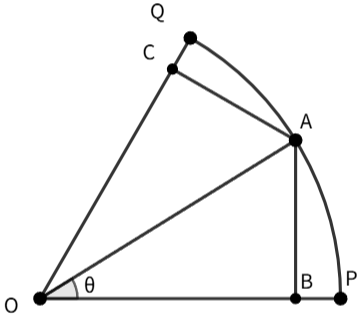
\includegraphics[width=5cm]{1.png}
        }
    \end{problemwithfig}
    % --- 修改结束 ---

\end{problems}

\end{document}